\section{Introduction}\label{intro}

In this project the main goal is to build a web application for student project allocation. Every year at the University of Southern Denmark, students from several different study programmes have to work on various projects relating to their specific study programme. For some of those projects the students are presented with a list of available topics, offered by their teachers. Each student, or group of students, must be assigned to a topic to work on. The allocation of the topics is based on the preferences of the students. Some of these cases involve hundreds of students and topics to be paired in a way that satisfies everyone involved, be it the teachers who offer the topics or the students who have to work on them.\\
To solve the problem of allocating students to topics an implementation of the algorithm described in \cite{Chiarandini2019} is used.\\The algorithm has been implemented as a python program, which currently runs as a console application. The users of the application has requested a user friendly interface to increase accessibility and usability, especially in relation to submitting projects and starting the allocation process. Visualising the results of the allocation was also requested as a way to show everyone involved that the assignment is in fact the most fair solution to a given case.
\\\\
The workflow for project allocation is as follows:\\
When the time comes for a group of students to select a project, they are presented with a list of all topics available. From this list each student, or group of students, selects the topics on which they wish to work, and submits a prioritized list of their chosen topics. At a predefined deadline the submitted lists are put in to the application, used for allocating and the results of this allocation is published. This workflow is visualised in Figure \ref{fig:intro_old}. The purpose of the web application is to automate as much of this workflow as possible.
\begin{figure}[b]
% \centering
\hrule
\vspace*{0.2cm}
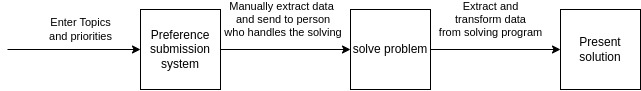
\includegraphics[width=0.9\textwidth]{workflow_old}
\caption{Diagram showing the workflow of the process of assigning students to topics}
\label{fig:intro_old}
% \hrule
\end{figure}
\begin{figure}[b!]
	\begin{tcolorbox}[title={Terminology in regards to the assignment program},colbacktitle=gray]
		\underline{\textit{Topic}}:\\A subject on which a student can work.\\
		\underline{\textit{Team}}:\\A group of students assigned to the same topic.\\
		\underline{\textit{Project}}:\\A specific instance of a Topic and a Team. e.g. Team ``a'' in Topic 7.\\
		\underline{\textit{Case}}:\\A collection of students and topics.\\
		\underline{\textit{Scenario}}:\\A specific assignment of students to projects in a case.\\
		\underline{\textit{Group}}:\\A set of students with the same preferences to be assigned to the same topic.\\
	\end{tcolorbox}
\label{text:termin_assignment}
\end{figure}
\\\\
In building the application I have used skills and knowledge gathered during the study of computer science at SDU.
\\\\While building a web application is in itself a complex task, a substantial part of this project has been the research of available tools and deciding why some were more suitable than others.
\\\\
Several sub-goals have been defined in order to break down the project into smaller and more accessible chunks, to more easily measure progress and provide a path from start to end. These sub-goals will constitute the chapters of this report.
\\\\
